\documentclass[12pt,fleqn]{article}
\setlength{\parindent}{0pt}
\usepackage{graphicx}
\usepackage{cancel}
\usepackage{listings}
\usepackage[latin5]{inputenc}
\usepackage{color}
\setlength{\parskip}{8pt}
\setlength{\parsep}{0pt}
\setlength{\headsep}{0pt}
\setlength{\topskip}{0pt}
\setlength{\topmargin}{0pt}
\setlength{\topsep}{0pt}
\setlength{\partopsep}{0pt}
\setlength{\mathindent}{0cm}

\begin{document}
Ders 1

Bir Kismi Turevsel Denklem (PDE) cok degiskenli bilinmeyen bir fonksiyon ve
o fonksiyonun kismi turevleri arasinda kurulan bir iliskidir. Mesela

\[ u = u(x,t) \]

olmak uzere

\[ \frac{\partial u}{\partial x} + \frac{\partial u}{\partial t} = 0\]

denklemi bir PDE'dir. Cozum bir tek sayisal sonuc degil, cozum bir
fonksiyon. Dusunelim, mesela $f$ fonksiyonu tek degiskenli ve turevi
alinabilir bir fonksiyon ise

\[ u(x,t) = f(x-t) \]

diyebilir miyiz? Yani cozum $f(x-t)$ olabilir mi? Kontrol edelim 

\[ u_x = f'(x-t) \]

\[ u_t = -f'(x-t) \]

Bu iki kismi turev toplaninca sifir cikar, yani sonuc ustte tanimli PDE'ye
uyar. Bu genel tanima uyan bir suru fonksiyon vardir, mesela 

\[ u(x,t) = (x-t)^2 \]

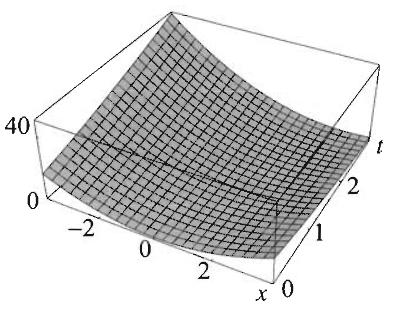
\includegraphics[height=4cm]{1_01.png}

\[ u(x,t) = e^{-(x-t)^2} \]

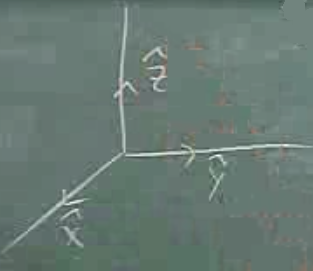
\includegraphics[height=4cm]{1_02.png}
















\end{document}
